\section{Experiments}
\label{sec:experiments}

Our experiments answer five questions in order. Does the substitution of
Section~\ref{sec:substitution} actually remove the divergence it was designed to
remove (\S\ref{sec:exp-diverge})? Is the resulting object a measure
(\S\ref{sec:exp-calib})? Does it serve rewards it never saw
(\S\ref{sec:exp-l2})? Is the residual error the one the theory predicted
(\S\ref{sec:exp-scale})? And can the prediction be acted on
(\S\ref{sec:exp-rewardz})? Section~\ref{sec:exp-suite} then reports where the
advantage stops.

\paragraph{Protocol.}
Unless stated otherwise: bilinear critic with $d=50$, twin heads with $\min$
backup, $\gamma=0.99$, $\epsilon=4$\,cm, hindsight-relabeled batch goals giving
$n\times n$ residuals, a flow-BC actor with one-step distillation, 500k gradient
steps, and 2--3 seeds per cell. Two evaluation harnesses recur. \emph{Native
goal-conditioned success} is the mean over the five built-in tasks, 50 episodes
each; it scores the \emph{actor}. \emph{Measure-side harnesses} score the learned
object directly and are described where first used. Section~\ref{sec:exp-calib}
shows these two families of number can disagree, which is why we report both.

% =====================================================================
\subsection{The bounded objective trains where the density form diverges}
\label{sec:exp-diverge}

Section~\ref{sec:singular} predicts a specific failure: with the orthonormality
anchor removed, the unmatched linear term should drive the diagonal of the density
estimator upward without bound. To rule out representation quality as an
explanation, we run both estimators on a \emph{frozen} backward map taken from a
checkpoint that already supports $0.97$ control.

The prediction holds (Figure~\ref{fig:diverge}). The density estimator's critic scale inflates from $154$ to
$5.4\times10^{4}$ within 65k steps and control decays $0.98\to0.42$ by 100k
(3 seeds), while the bounded estimator on the same frozen embedding plateaus on
the Monte-Carlo estimate of the true visitation mass --- it converges to the
correct magnitude rather than to a rescaled surrogate. Both stabilizers of
Equation~\ref{eq:fb-loss} are independently harmful: removing
$\mathcal{L}_{\mathrm{ortho}}$ gives the divergence above, while retaining it
bounds the scale but suppresses control to $0.225$. Removing \emph{both} --- which
the substitution permits, since the $0/1$ target supplies the anchor the
regularizer stood in for --- reaches $0.967$, above the matched goal-conditioned
anchor at $0.928$ and more than double the $0.42$ of vanilla FB.
Appendix~\ref{app:diverge} gives the full control set, and
Appendix~\ref{app:playpen} reproduces the same separation exactly in a $50$-state
MDP where both estimators can be solved in closed form.

\begin{figure}[t]
\centering
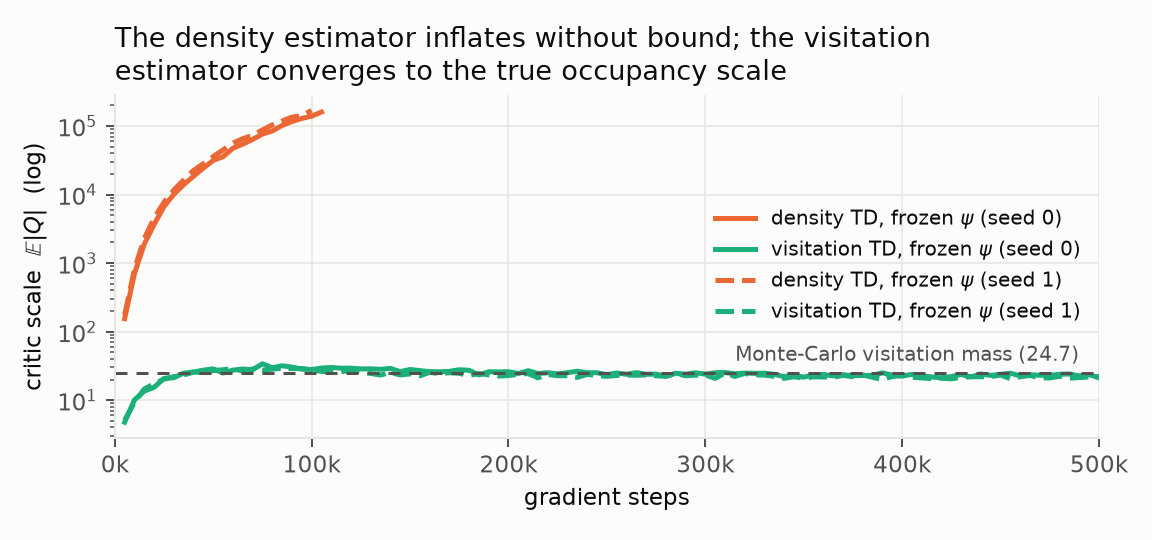
\includegraphics[width=0.66\textwidth]{figures/scale_divergence.png}
\caption{Critic scale $\E|Q|$ (log) during visitation-style training on a
\emph{frozen} phase-1 embedding. The density estimator (orange) inflates without
bound once the orthonormality anchor is removed --- its linear term pays
unconditionally for larger $M$. The bounded region estimator (aqua) plateaus on
the Monte-Carlo estimate of the true discounted visitation mass (dashed): it
converges to the measure, not to a rescaled surrogate.}
\label{fig:diverge}
\end{figure}

\begin{takeaway}
The divergence is a property of the estimator, not of the representation: it
occurs on a frozen embedding that supports $0.97$ control. Orthonormality and the
linear diagonal term are load-bearing in opposite directions, and the bounded
target removes the need for either, reaching $0.967$ against a $0.928$
goal-conditioned anchor. This is a claim about the value objective only --- all
cells share one actor class.
\end{takeaway}

% =====================================================================
\subsection{The learned object is a measure at set level, but not pointwise}
\label{sec:exp-calib}

Task success cannot answer this question. The actor consumes only
$\arg\max_a\langle F,z\rangle$ --- an ordering over actions at a single state ---
so a critic can order actions perfectly while being an arbitrary function of $g$.
The two properties are logically independent, and on our own checkpoints they come
apart: over a grid of $24$ states $\times$ $150$ goals $\times$ $16$ actions, the
reaching value and the visitation measure agree on the greedy action only
$29.5\%$/$29.9\%$ of the time (2 seeds). Chance on this action set is $6.25\%$, so
the agreement is well above chance but far below the $0.9$ a shared argmax would
imply. A high success rate certifies $Q$, not $M$.

\paragraph{Set-mass calibration.}
We compare the model's mass on random boxes against Monte-Carlo occupancy of the
same boxes under the policy being scored, from $32$ start states $\times$ $3$
rollouts at horizon $200$. We report the denominator two ways: exact kernel counts
$\rho(B_\epsilon(g))$, which isolate the error in $M$ itself, and the trained
$\hat N$ head, which scores the deployed object end to end.

\begin{table}[t]
\centering\footnotesize
\begin{tabular}{c c c c c}
\toprule
& & \multicolumn{2}{c}{model / MC} & \\
\cmidrule(lr){3-4}
half-width & MC mass & exact $\rho$ & trained $\hat N$ & Spearman \\
\midrule
$0.4$ & $0.56/0.86$ & $3.22/2.03$ & $1.94/1.22$ & $+0.31/+0.33$ \\
$0.8$ & $5.98/5.82$ & $1.92/2.08$ & $\mathbf{1.10/1.16}$ & $+0.68/+0.72$ \\
$1.6$ & $27.4/28.1$ & $2.33/2.18$ & $\mathbf{1.23/1.14}$ & $+0.85/+0.82$ \\
\bottomrule
\end{tabular}
\caption{Set-mass calibration of the phase-2 object, per seed. At the two coarser
scales the deployed object is within $10$--$23\%$; multiplying by the truncation
factor $1-\gamma^{H}=0.87$ brings it to ${\approx}1.0$.}
\label{tab:calib}
\end{table}

At half-widths $0.8$ and $1.6$ the deployed object is calibrated to within
$10$--$23\%$ and orders regions at Spearman $0.68$--$0.85$. Accounting for the
horizon --- the model estimates an infinite-horizon mass while the Monte-Carlo sum
stops at $H{=}200$, discarding $\gamma^{H}=0.134$ --- brings the ratio to
approximately $1.0$. At set level, on this environment, the object behaves like a
measure.

Three qualifications keep that from being stronger than it is. The calibrated
column divides by the \emph{trained} $\hat N$; with exact counts the same object is
$1.9$--$3.2\times$ off, and since the head over-predicts density by $28\%$, part of
the agreement is two biases cancelling. Calibration degrades at the smallest scale
($1.2$--$1.9\times$, Spearman $0.32$), which is the radius of the training kernel
itself --- the object is weakest at the resolution it was fit at. And all of this
is one environment.

\paragraph{Pointwise, it is not a measure.}
Over $8$ draws of $(s_0,a_0,z)$ per seed against 100k goal states,
$\Pr[M<0] = 45.0\%/45.9\%$. A successor measure is non-negative by definition, so
pointwise the object fails, even where its set-level mass is right: negative
entries cancel against positive ones inside a box, which is exactly how aggregate
calibration can look good while the allocation underneath is wrong.

The obvious repair trades one defect for another. Adding a one-sided squared hinge
$\lambda\,\E[\mathrm{relu}(-M)^2]$ --- a penalty rather than a softplus or squared
parameterization, so that $M$ stays linear in $\psi$ and the $\langle F,z_r\rangle$
readout survives --- removes the negative mass ($45\%\to3.1\%$ at $\lambda{=}1$,
$\to0.7\%$ at $\lambda{=}10$) at no cost in task success. But it inflates set mass
monotonically in $\lambda$, to $2.5$--$3.6\times$ at half-width $0.8$ against the
unpenalized $1.10/1.16$: the hinge pushes negatives up with nothing conserving
total mass. We do not adopt it.

\begin{takeaway}
Set-level mass and coarse ordering are calibrated ($1.10$--$1.23\times$,
$\rho=0.68$--$0.85$); pointwise values are not ($45\%$ negative). The two coexist
because signs cancel within a box. Every intervention we tried trades one against
the other, so a mass-conserving route to non-negativity remains open. Note also
that the calibrated numbers rely on a learned density head whose own bias
partially cancels the error.
\end{takeaway}

% =====================================================================
\subsection{It serves rewards it never saw, and it composes}
\label{sec:exp-l2}

Section~\ref{sec:exp-calib} leaves a split verdict, so we test the readout
directly on rewards absent from training. All rewards are functions of the cube
position; centers are drawn from dataset states so every reward is supported on
visited space. Six families $\times$ $8$ instances $=48$ rewards sweep the
reward's spatial support outward from the kernel's own radius: indicator balls at
$\epsilon\in\{0.4,0.8,1.6\}$ (in observation units, where the trained kernel is
$0.4$), Gaussians at $\sigma\in\{0.4,0.8\}$ with no support boundary at all, and a
two-zone family placing two disjoint balls more than $1.6$ apart, which no single
goal can express. A task vector is inferred by the moment readout on $m{=}10{,}000$
relabeled rows with no ridge, no $\hat N$ correction and no policy improvement over
candidates --- the minimal pipeline, so that what is tested is the representation
rather than a decoder.

\paragraph{Baselines.}
We report a normalized gap
$(G_{z_r}-G_{\mathrm{floor}})/(G_{\mathrm{ceil}}-G_{\mathrm{floor}})$ against three
references, and we are explicit about them because the choice of floor changes the
reading. The \emph{ceiling} is $\psi$ of the dataset state nearest the reward's
center, an oracle handed the answer; it is a proxy, since ``go to the center'' is
not optimal for a broad Gaussian, and it therefore understates performance on
exactly the widest families. The \emph{floor} is a random task vector driving the
same actor. The \emph{behavior} baseline is the return the offline data itself
earns. On concentrated families the last two agree closely ($1.21$ vs $0.91$ on
\textsc{ball}~$0.4$), but on broad ones they diverge sharply: on
\textsc{ball}~$1.6$ the data earns $25.1$ while a \emph{random} task vector earns
$35.6$, because a $16$\,cm ball rewards an actor that merely moves the cube. We
report both normalizations.

\begin{table}[t]
\centering\footnotesize
\begin{tabular}{l c c c c}
\toprule
& \multicolumn{2}{c}{prediction} & \multicolumn{2}{c}{control (gap)} \\
\cmidrule(lr){2-3}\cmidrule(lr){4-5}
Family & Spearman & scale & vs.\ random $z$ & vs.\ behavior \\
\midrule
\textsc{ball} $0.4$   & $0.85/0.90$ & $0.014$ & $0.87/0.74$ & $0.80$ \\
\textsc{ball} $0.8$   & $0.80/0.81$ & $0.023$ & $0.70/0.61$ & $0.65$ \\
\textsc{twozone}      & $0.73/0.69$ & $0.017$ & $\mathbf{0.83/0.89}$ & $\mathbf{0.86}$ \\
\textsc{smooth} $0.4$ & $0.75/0.86$ & $0.019$ & $0.54/0.46$ & $0.52$ \\
\textsc{smooth} $0.8$ & $0.62/0.75$ & $0.018$ & $0.23/0.08$ & $0.32$ \\
\textsc{ball} $1.6$   & $0.72/0.81$ & $0.018$ & $-0.10/0.24$ & $0.44$ \\
\bottomrule
\end{tabular}
\caption{Transfer to $48$ never-trained rewards, eval-only. Prediction scale is
$\E[\text{predicted}]/\E[\text{Monte Carlo}]$, target $1$.}
\label{tab:l2}
\end{table}

Concentrated rewards reach $0.66$--$0.86$ of the oracle, and \textsc{twozone} ---
two disjoint targets --- is the \emph{strongest} family. Transfer degrades as the
reward's bandwidth grows. Ordering, however, is uniformly good: Spearman stays
$0.62$--$0.90$ across every family, including the ones where control collapses.
The object ranks returns correctly on rewards it cannot act on.

\paragraph{Does the visitation backup earn its keep?}
The gap in Table~\ref{tab:l2} is normalized \emph{within} a checkpoint, against
that checkpoint's own oracle and floor, so it cannot be used to rank methods:
oracle ceilings differ across methods by up to $2\times$ on identical rewards, and
a method with a weaker oracle scores higher while earning less. We therefore
compare absolute discounted return, running the reaching backup of
Equation~\ref{eq:backups} and FB's own loss at matched support through the
identical harness.

\begin{center}\footnotesize
\begin{tabular}{l c c c c}
\toprule
& \textsc{ball} $0.4$ & \textsc{twozone} & \textsc{smooth} $0.8$ & mean (6 families) \\
\midrule
reaching backup       & $10.01$ & $8.45$  & $19.71$ & $16.75$ \\
FB loss, matched support & $1.52$ & $4.96$ & $16.43$ & $13.09$ \\
visitation backup     & $\mathbf{15.57}$ & $\mathbf{15.82}$ & $19.43$ & $\mathbf{20.26}$ \\
\bottomrule
\end{tabular}
\end{center}

The visitation backup earns $1.33\times$ the reaching backup's return on average
and up to $1.87\times$ on \textsc{twozone}, and the mechanism is visible in the
oracle ceilings: driven to the \emph{same} goal with the answer supplied, the
visitation policy accumulates $1.13$--$2.00\times$ more reward than the reaching
policy. A reaching value saturates on arrival, so its policy arrives and stops; a
visitation policy stays. The advantage is largest on concentrated and
compositional rewards ($1.56\times$, $1.87\times$) and vanishes on broad ones
($0.99\times$, $1.05\times$), which is consistent --- a reward earned by wandering
gains nothing from dwelling. FB's loss at matched support is worst of the three
and on two families its oracle drive earns \emph{less} than a random task vector,
so it yields no usable readout at all.

One confound: the visitation checkpoint is warm-started from the reaching one and
trained for a further 500k steps, so it has twice the budget. The ceiling
comparison is less exposed to this, since it measures what each policy class
accumulates when handed the goal, but an iso-budget control is owed.

\begin{takeaway}
The measure serves unseen rewards zero-shot and composes over disjoint regions,
and it earns $1.33\times$ the return of a reaching value trained identically ---
because a reaching value's policy arrives and stops while a visitation policy
dwells. This is the first direct evidence that the visitation backup buys the
semantics it was introduced for. The comparison is not iso-budget, and all
families are functions of the same privileged coordinate, so these are novel
rewards over a given abstraction rather than novel abstractions.
\end{takeaway}

% =====================================================================
\subsection{The scale error is exactly the missing normalization}
\label{sec:exp-scale}

The scale column of Table~\ref{tab:l2} is the interesting one. Predicted
magnitudes are $0.014$--$0.030$ of the truth in \emph{every} family, a constant
offset rather than a family-dependent error. Section~\ref{sec:owed} predicted
this before the experiment was run, and predicted its size: a readout omitting
$1/\hat N$ should be wrong by the mean region mass $\bar N$. Measured
independently on the same checkpoints, $\bar N = 0.0137$. The agreement is exact
on \textsc{ball}~$0.4$ ($0.0136$) and within a factor of two on every other
family.

\begin{figure}[t]
\centering
\includegraphics[width=0.45\textwidth]{figures/scale.pdf}
\caption{Predicted against true return for all $48$ transfer rewards, log-log.
The naive readout tracks $y=\bar N x$ for the independently measured
$\bar N = 0.0137$ --- the density division Section~\ref{sec:owed} predicted it
omits --- while the $1/\hat N$-weighted readout tracks $y=x$.}
\label{fig:scale}
\end{figure}

Re-running inference with weights $1/\hat N$ confirms the mechanism directly
(Figure~\ref{fig:scale}):
prediction scale moves from $0.014$--$0.030$ to $0.79$--$2.2$, meeting the gate.
The debt incurred by the region substitution is therefore real, quantified, and
repayable.

What the correction does \emph{not} do is improve control. Under the same
weighting, control is unimproved everywhere and \emph{regresses} where it worked:
\textsc{twozone} falls $0.86\to0.46$ and \textsc{ball}~$0.8$ falls $0.65\to0.48$.
Prediction and control want different readouts --- naive $z_r$ for acting,
$1/\hat N$-weighted for integrating --- which is a symptom rather than a design.
It also localizes the residual defect away from the inference rule: if a better
$z_r$ makes returns more predictable but behavior no better, the limitation is in
what the actor can do with $z_r$, not in how $z_r$ is computed. The trained task
distribution is $50\%$ random directions and $50\%$ $\psi$ of a single goal; a
broad reward's $z_r$ is an average of many $\psi$'s and lies off both.

\begin{takeaway}
The readout's scale error equals the mean region mass $\bar N=0.0137$ that
Section~\ref{sec:owed} predicted, and $1/\hat N$ weighting repairs prediction. It
does not repair control, which localizes the remaining defect to the actor's
task-vector manifold rather than to inference. The prediction was made before the
measurement, but on the same environment that motivated the theory.
\end{takeaway}

% =====================================================================
\subsection{Broad rewards need a populated task-vector manifold}
\label{sec:exp-rewardz}

That diagnosis is testable by changing the training task distribution and nothing
else. We add a third component to the $z$ law, drawn exactly as the zero-shot
readout draws it --- $z=\Pi(\sum_i r_i\psi(x_i))$ for a random synthetic reward
over the batch --- at mixing fraction $\eta$, holding phase 1, the objective, and
every other hyperparameter fixed, and warm-starting from the same phase-1
checkpoints as the control. Thresholds were registered before the runs.

Two reward generators are deliberately distinguished. \textsc{kernel} draws balls,
Gaussians and two-zone rewards with random centers and log-uniform radii: the
evaluation families' \emph{functional form}, so it upper-bounds what the actor can
learn. \textsc{rff} draws $r=\mathrm{relu}(\cos(w^{\top}\cube+\varphi))$ with
$w\sim\mathcal{N}(0,I)/b$ --- non-negative random fields of controlled length
scale, a \emph{different} functional form, so the evaluation families stay held out
and a win cannot be an artifact of training on the test distribution.

\begin{table}[t]
\centering\footnotesize
\begin{tabular}{l c c c c}
\toprule
Family & control & \textsc{kernel} $\eta{=}0.25$ & \textsc{kernel} $\eta{=}0.5$ & \textsc{rff} $\eta{=}0.25$ \\
\midrule
\textsc{ball} $0.4$   & $0.80$ & $0.87$ & $0.87$ & $0.79$ \\
\textsc{ball} $0.8$   & $0.66$ & $0.71$ & $\mathbf{0.95}$ & $0.73$ \\
\textsc{twozone}      & $0.86$ & $0.92$ & $\mathbf{1.35}$ & $1.11$ \\
\textsc{smooth} $0.4$ & $0.50$ & $0.49$ & $\mathbf{0.78}$ & $0.55$ \\
\textsc{smooth} $0.8$ & $0.15$ & $0.27$ & $0.33$ & $0.12$ \\
\textsc{ball} $1.6$   & $0.07$ & $\mathbf{0.53}$ & $\mathbf{0.49}$ & $\mathbf{0.55}$ \\
\midrule
mean (all 6)          & $0.507$ & $0.630$ & $\mathbf{0.795}$ & $0.640$ \\
task success          & $0.887$ & $0.948$ & $0.950$ & $0.930$ \\
set mass @ hw $0.8$   & $1.10/1.16$ & $1.10/1.19$ & $1.23/1.31$ & $1.26/1.12$ \\
\bottomrule
\end{tabular}
\caption{Populating the task-vector manifold. Control gap vs.\ random $z$, 2-seed
means, with both pre-registered guards.}
\label{tab:rewardz}
\end{table}

\begin{figure}[t]
\centering
\includegraphics[width=\textwidth]{figures/bandwidth.pdf}
\caption{Zero-shot control against the reward's spatial support. Transfer
degrades as support widens (left to right within each family); training on
synthetic-reward task vectors repairs the wide \emph{indicator} rewards and the
compositional family, but not the wide Gaussian. The held-out reward form
(\textsc{rff}) performs comparably to the matched one, so the effect is coverage
of the task-vector manifold rather than familiarity with the test distribution.}
\label{fig:bandwidth}
\end{figure}

The registered primary read --- broad families above $0.4$ while concentrated ones
hold above $0.7$ --- is half met, informatively (Figure~\ref{fig:bandwidth}). \textsc{ball}~$1.6$ clears
decisively, from $-0.10/0.24$ to $0.47$--$0.55$ on every arm and both seeds, while
\textsc{smooth}~$0.8$ does not, topping out at $0.33$. Broad \emph{indicator}
rewards are repaired; broad \emph{Gaussian} rewards are not, and the difference
between them is that a Gaussian has no support boundary, so its $z_r$ averages
essentially the whole dataset. Both guards pass: task success does not degrade but
improves ($0.887\to0.93$--$0.95$), and set-mass calibration is unchanged.

Two structural points. The mechanism is confirmed --- because the matched-form arm
works, the actor's task-vector manifold really was the binding constraint, which
Section~\ref{sec:exp-scale} inferred rather than showed. And the result is not
circular: \textsc{rff}, sharing no functional form with any evaluation family,
matches or beats the matched arms on \textsc{ball}~$1.6$. What the $z$ law supplies
is coverage of the broad-$z$ region, not familiarity with the test distribution.
Finally, \textsc{twozone} at $1.35$ exceeds the single-goal oracle ceiling by
$35\%$, as a genuine measure should, since that ceiling is the better of the two
zones alone.

\begin{takeaway}
Training on synthetic-reward task vectors raises overall zero-shot control from
$0.507$ to $0.795$ without cost to task success or calibration, converting a
diagnosed defect into a repair. A held-out reward form works as well as the
matched one, so the effect is coverage rather than test-set familiarity. Broad
Gaussians remain unsolved, and this arm has 2 seeds.
\end{takeaway}

% =====================================================================
\subsection{The advantage does not survive off \texttt{cube-single}}
\label{sec:exp-suite}

Every measure-side result above is one environment. We extend both backups to the
four OGBench state-based manipulation environments for which a tuned vanilla-FB
number exists, against a goal-conditioned anchor matched in data, actor class,
critic rank and budget.

\begin{table}[t]
\centering\footnotesize
\begin{tabular}{l c c c}
\toprule
Environment & reaching (phase 1) & visitation (phase 2) & GC-IQL anchor \\
\midrule
\texttt{cube-single} & $\mathbf{0.967}$ & $0.940$ & $0.928$ \\
\texttt{cube-double} & $\mathbf{0.549}$ & $0.358$ & $0.265$ \\
\texttt{scene}       & $\mathbf{0.484}$ & $0.342$ & $0.281$ \\
\texttt{puzzle-3x3}  & $0.200$ & $0.198$ & $0.117$ \\
\bottomrule
\end{tabular}
\caption{Overall success at 500k, 2--3 seeds. \texttt{puzzle-3x3} is degenerate:
every seed scores $1.0$ on task~1 and $0.0$ on tasks~2--5, so the margin is one
task's, and no method here solves the other four.}
\label{tab:suite}
\end{table}

The reaching backup exceeds its matched anchor on all four environments --- by
$2.1\times$ and $1.7\times$ on the two harder ones --- and since the anchor shares
data, actor class, critic rank and budget, the objective is what differs. The
visitation backup does not hold that level: it costs $0.19$ on
\texttt{cube-double} and $0.14$ on \texttt{scene} while \texttt{cube-single} stays
roughly flat. It still clears the anchor everywhere, so the curriculum is not
broken, but the reading that the visitation phase is free does not survive off
\texttt{cube-single}. Absolute numbers also fall away for every method as the goal
region becomes a conjunction over more objects, which bounds what any of these
numbers say about manipulation in general.

\begin{takeaway}
The reaching backup's advantage over a matched goal-conditioned anchor holds on
all four environments; the visitation backup's does not, costing $0.19$ and $0.14$
on the two harder ones. Since the visitation backup is the one that yields a
measure, the capability of Sections~\ref{sec:exp-l2}--\ref{sec:exp-rewardz} is
currently demonstrated only where it is also free.
\end{takeaway}
